% !TEX root = ./main.tex
% !TEX encoding = UTF-8 Unicode
% !TEX program = pdflatex
% !TeX spellcheck = it_IT

\graphicspath{{Immagini/},{Immagini/ffda/}}

\chapter{Field Failure Data Analysis}
La \textbf{FFDA} è effettuata sui dati relativi ad un sistema in
esercizio(\textit{on Field}), al fine di scoprire i possibili fallimenti.\\
L'approccio utilizzato nella FFDA prevede di monitorare il sistema in esecuzione,
misurando parametri di dependability e prelevando tutte le possibili informazioni
sul fallimenti rilevati.\\
Un fallimento è una deviazione del comportamento del sistema dal suo corretto e
specifico funzionamento.\\
La metodologia FFDA è basata su tre fasi fondamentali:
\begin{itemize}
  \item \textbf{Data Logging \& Collection} - consiste nella definizione di cosa
  collezionare e come farlo;
  \item \textbf{Data Filtering \& Manipulation} - consiste nella manipolazione ù
  dei dati collezionati, utilizzando \textit{filtering} e \textit{coalescence};
  \item \textbf{Data Logging \& Collection} - consiste nell'esecuzione di un'analisi
  statistica su dati precedentemente manipolati, per calcolarne misure quantitative
  e identificarne possibili trends.\\
\end{itemize}

\section{Traccia}
Dati i due file di log \textit{MercuryErrorLog} e \textit{BGLErrorLog},
preventivamente filtrati per ottenere solo eventi di fallimento, si vuole:
\begin{itemize}
  \item determinare la finestra di coalescenza;
  \item raggruppare tutte le entry appartenenti alle stesse finestre di
  coalescenza(tuple);
  \item ricavare la \textit{CDF} del \textbf{TTF}(Time-To-Failure) e della
  \textbf{Reliability Empirica};
  \item fitting della CDF della reliability empirica provando tutti i modelli
  studiati (\textit{Esponenziale}, \textit{Weibull} ed \textit{Iperesponenziale});
  \item utilizzare il test di \textit{Kolmogorov-Smirnov} per controllare che il
  modello ipotizzato fitti adeguatamente i dati.\\
\end{itemize}

\clearpage

\section{Mercury}
Il sistema Mercury consiste di nodi IBM.\\
Il cluster ha un'architettura a 3 livelli(nodi \textit{login}, \textit{computation}
e \textit{storage}) ed un solo nodo di management
(\textit{tg-master}).\\
Il log è formato dai seguenti campi:
\begin{itemize}
  \item \textbf{Timestamp};
  \item \textbf{Nodo Origine};
  \item \textbf{Categoria Errore}:
  \begin{itemize}
    \item DEV, PRO, MEM, NET, IO, OTH;
  \end{itemize}
  \item \textbf{Messaggio}.
\end{itemize}

\subsection{Finestra di Coalescenza - CWIN}
La finestra di coalescence, definita in secondi, definisce un intervallo temporale
in cui cadono tutti gli eventi che vi appartengono.\\
Lo script \textbf{tupleCount\_func\_CWINpy.sh}(riportato in figura \ref{coalescence_window_mercury}), con input i file \textit{MercuryErrorLog.txt}
e \textit{tentative-CWIN.txt}, è stato utilizzato per calcolare il numero di tuple al
variare della dimensione della finestra di coalescenza.\\

\begin{figure}[!htbp]
  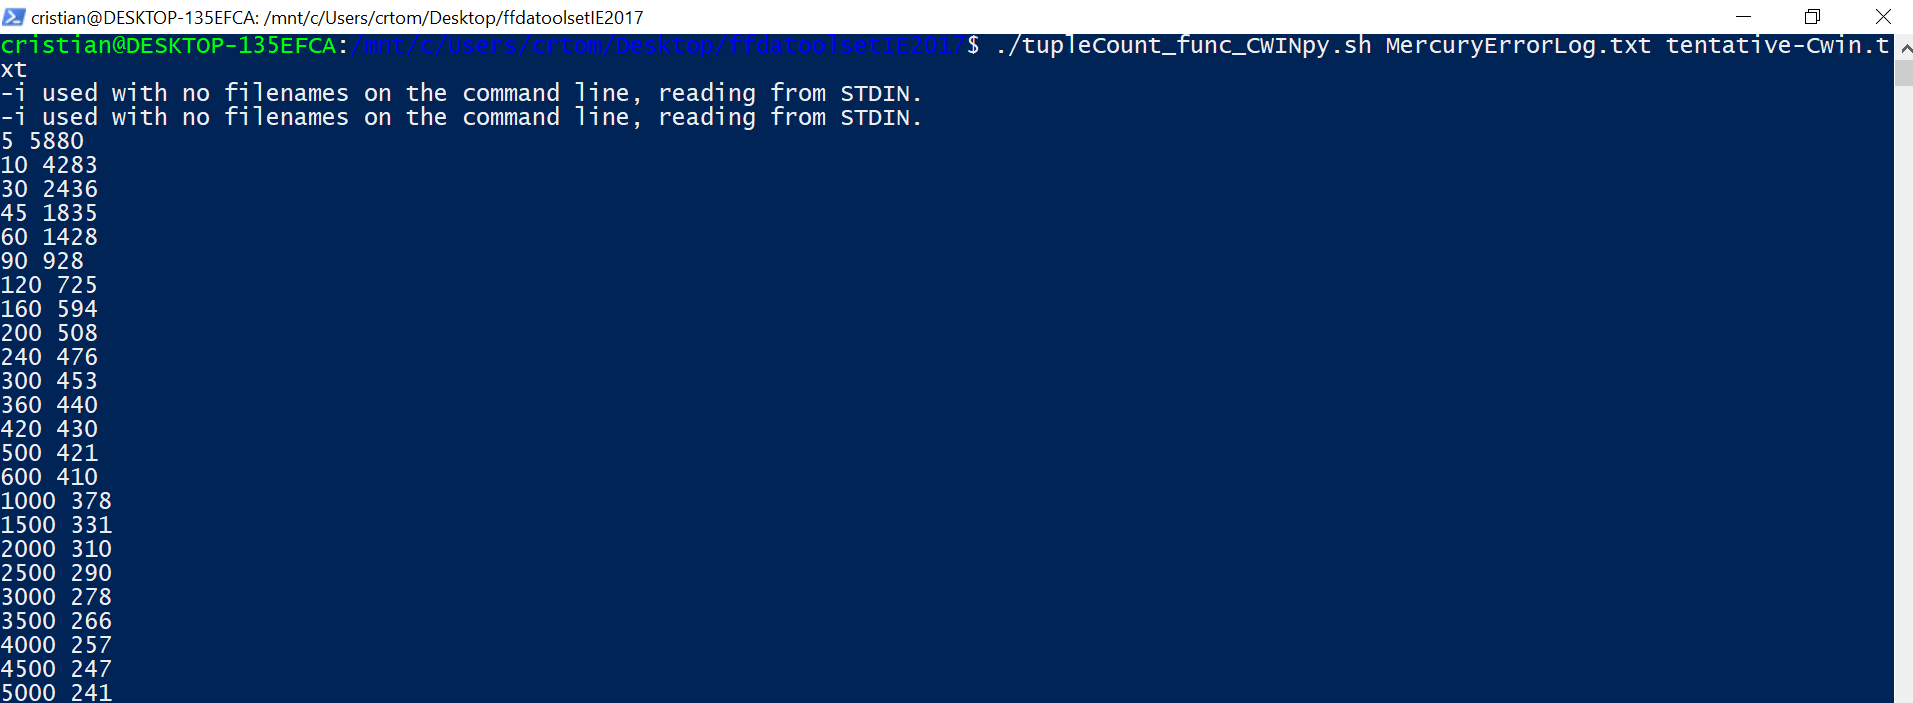
\includegraphics[width=1\linewidth,keepaspectratio]{coalescence_window_mercury}
  \caption{Script conteggio tuple al variare della finestra di coalescenza}
  \label{coalescence_window_mercury}
\end{figure}

\clearpage

L'output di tale script, plottato in matlab e presente in figura \ref{plot_coalescence_window_mercury},
è infine utilizzato per determinare un singolo valore di CWIN, ottenuto
considerando il punto successivo al ginocchio(knee) della curva.\\
Il valore di CWIN scelto è 300.\\
\begin{figure}[!htbp]
  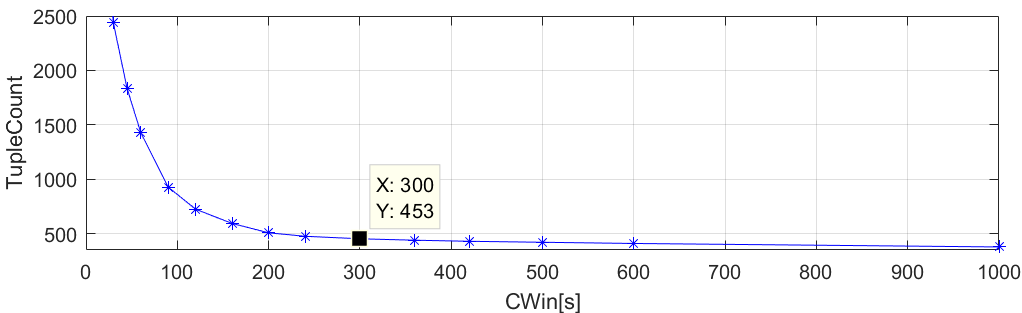
\includegraphics[width=1\linewidth,keepaspectratio]{plot_coalescence_window_mercury}
  \caption{Plot finestre di coalescenza}
  \label{plot_coalescence_window_mercury}
\end{figure}

%%ANDREA è ARRAIVATO QUI!!!
Lo script bash \textbf{tupling\_with\_CWIN.sh} suddivide le righe del file di log
secondo la finestra di coalescenza calcolando infine per ogni tupla si seguenti parametri:

\begin{itemize}
  \item \textbf{Starting Points}: il timestamp della prima riga di ogni tupla generata;
  \item \textbf{Interarrivals}: il tempo che intercorre, tra due tuple consecutive, tra l'ultimo
  della prima tupla e il primo della seconda;
  \item \textbf{Lenghts}: il numero di righe di ogni tupla.
\end{itemize}

Analizzando il file \textbf{interarrivals.txt} in matlab tramite lo script \textbf{ttf\_ref}
si ottiene la CDF empirica della TTF(Time To Failure) e dualmente la Reliability (1-TTF).\\
In figura è riportato il grafico delle due CDF.

\begin{figure}[!htbp]
  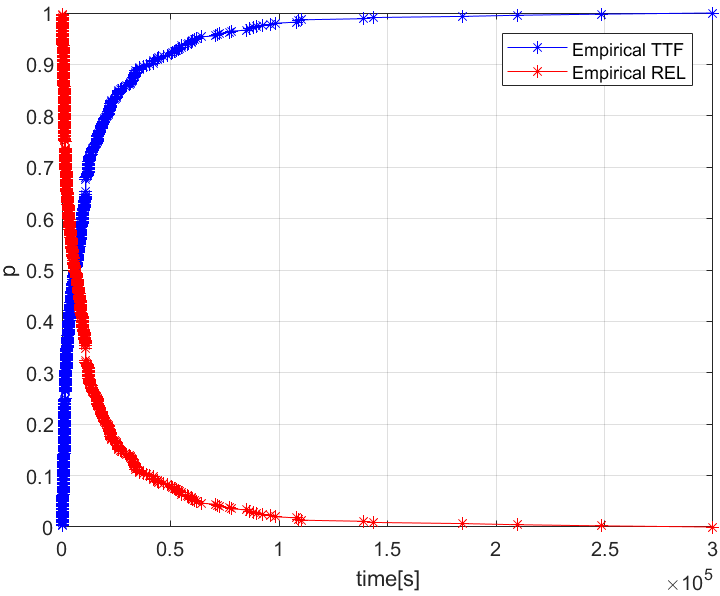
\includegraphics[width=1\linewidth,keepaspectratio]{ttf_rel_mercury}
  \caption{Plot TTF e Reliability}
  \label{ttf_rel_mercury}
\end{figure}

\section{Curve Fitting}

Dopo aver ottenuto la CDF della reliability è possibile procedere con fitting.\\
Utilizzando il tool di matlab \textbf{Curve Fitting} è stato possibile
analizzare i seguenti modelli:

\clearpage

\begin{itemize}
  \item \textbf{Esponenziale}:
  $$ y = e^{- \lambda  x} $$
  Il valore $\lambda$ è stato inizializzato a $1/MTTF$.\\
  Il modello risultante in matlab è riportato nella figura \ref{Exponential_mercury}.\\

  \begin{figure}[!htbp]
    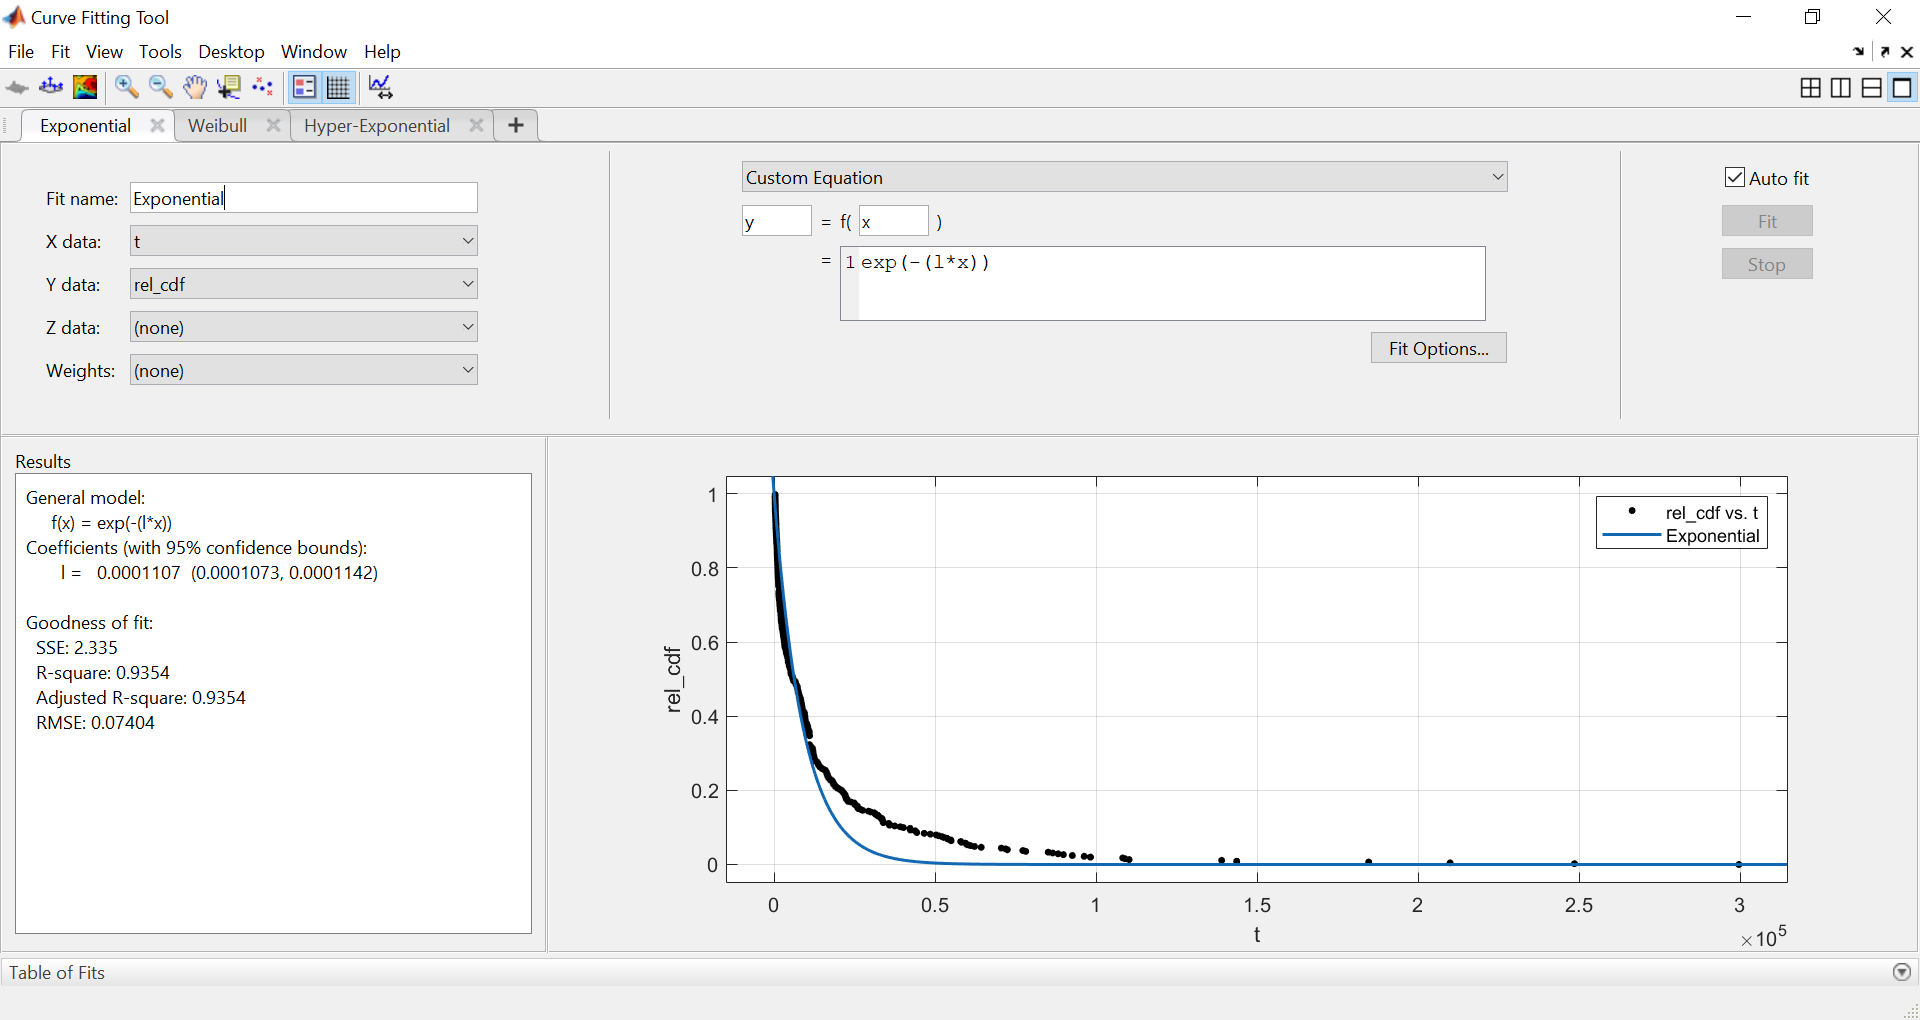
\includegraphics[width=.9\linewidth,keepaspectratio]{Exponential_mercury}
    \caption{Curve Fitting modello esponenziale}
    \label{Exponential_mercury}
  \end{figure}

  Per valutare la bontà del fitting è stato utilizzato il \textbf{Kolmogorov-Smirnov Test}.\\

  \begin{figure}[!htbp]
    \centering
    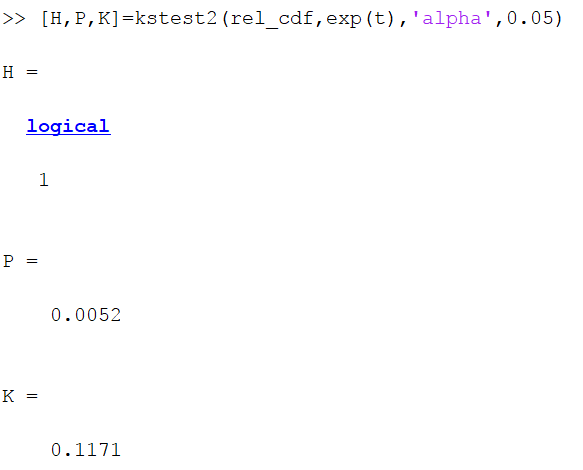
\includegraphics[width=0.5\linewidth,keepaspectratio]{ks_exp_mercury}
    \caption{Kolmogorov-Smirnov Test esponenziale}
    \label{ks_exp_mercury}
  \end{figure}

  L'ipotesi nulla è rigettata al 99,48\% con un intervallo di confidenza al 95\%.

  \clearpage

  \item \textbf{Weibull}:
  $$ y = e^{- (\lambda x)^\alpha} $$
  Il modello risultante in matlab è riportato nella figura \ref{Weibull_mercury}.\\
  \begin{figure}[!htbp]
    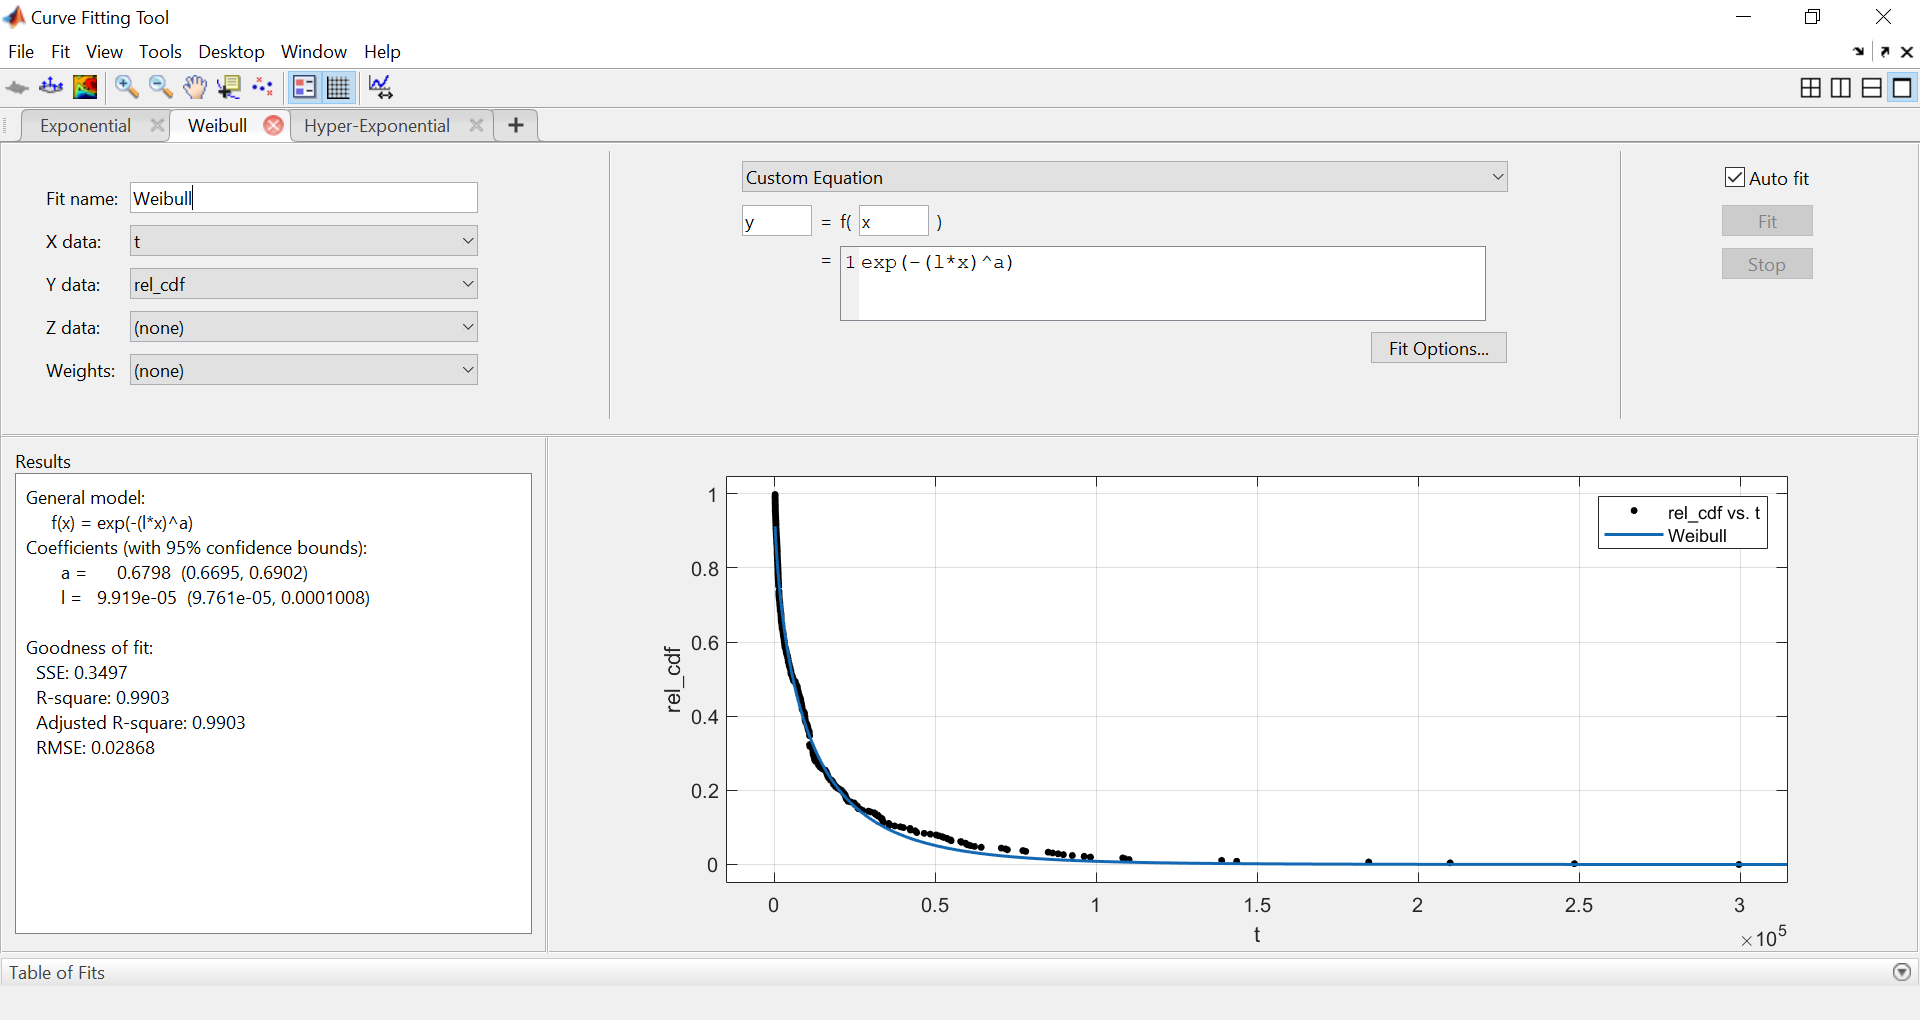
\includegraphics[width=0.9\linewidth,keepaspectratio]{Weibull_mercury}
    \caption{Curve Fitting modello esponenziale}
    \label{Weibull_mercury}
  \end{figure}

  Per valutare la bontà del fitting è stato utilizzato il \textbf{Kolmogorov-Smirnov Test}.\\

  \begin{figure}[!htbp]
    \centering
    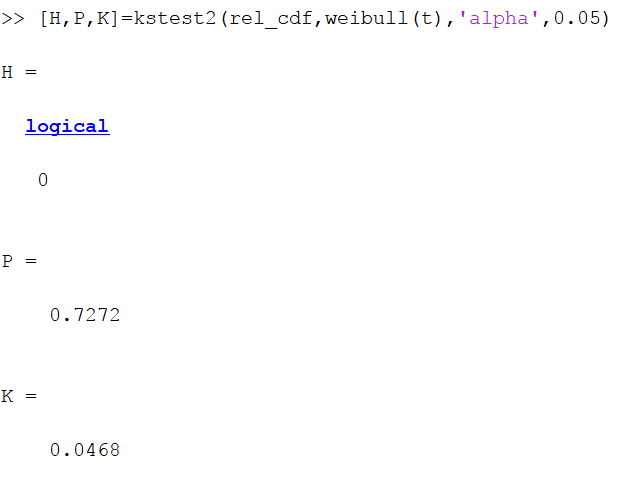
\includegraphics[width=0.5\linewidth,keepaspectratio]{ks_weibull_mercury}
    \caption{Kolmogorov-Smirnov Test Weibull}
    \label{ks_weibull_mercury}
  \end{figure}

  L'ipotesi nulla non è rigettata al 72,72\% con un intervallo di confidenza al
  95\% quindi osservando il anche il valore di R-quadro si può concludere che il
  modello ipotizzato fitta bene la CDF empirica.\\

  \clearpage

  \item \textbf{Iperesponenziale}:
  $$ y = a e^{- \lambda_1  x} +  b  e^{- \lambda_2  x} $$
  Il modello risultante in matlab è riportato nella figura \ref{HyperExponential_mercury}.\\

  \begin{figure}[!htbp]
    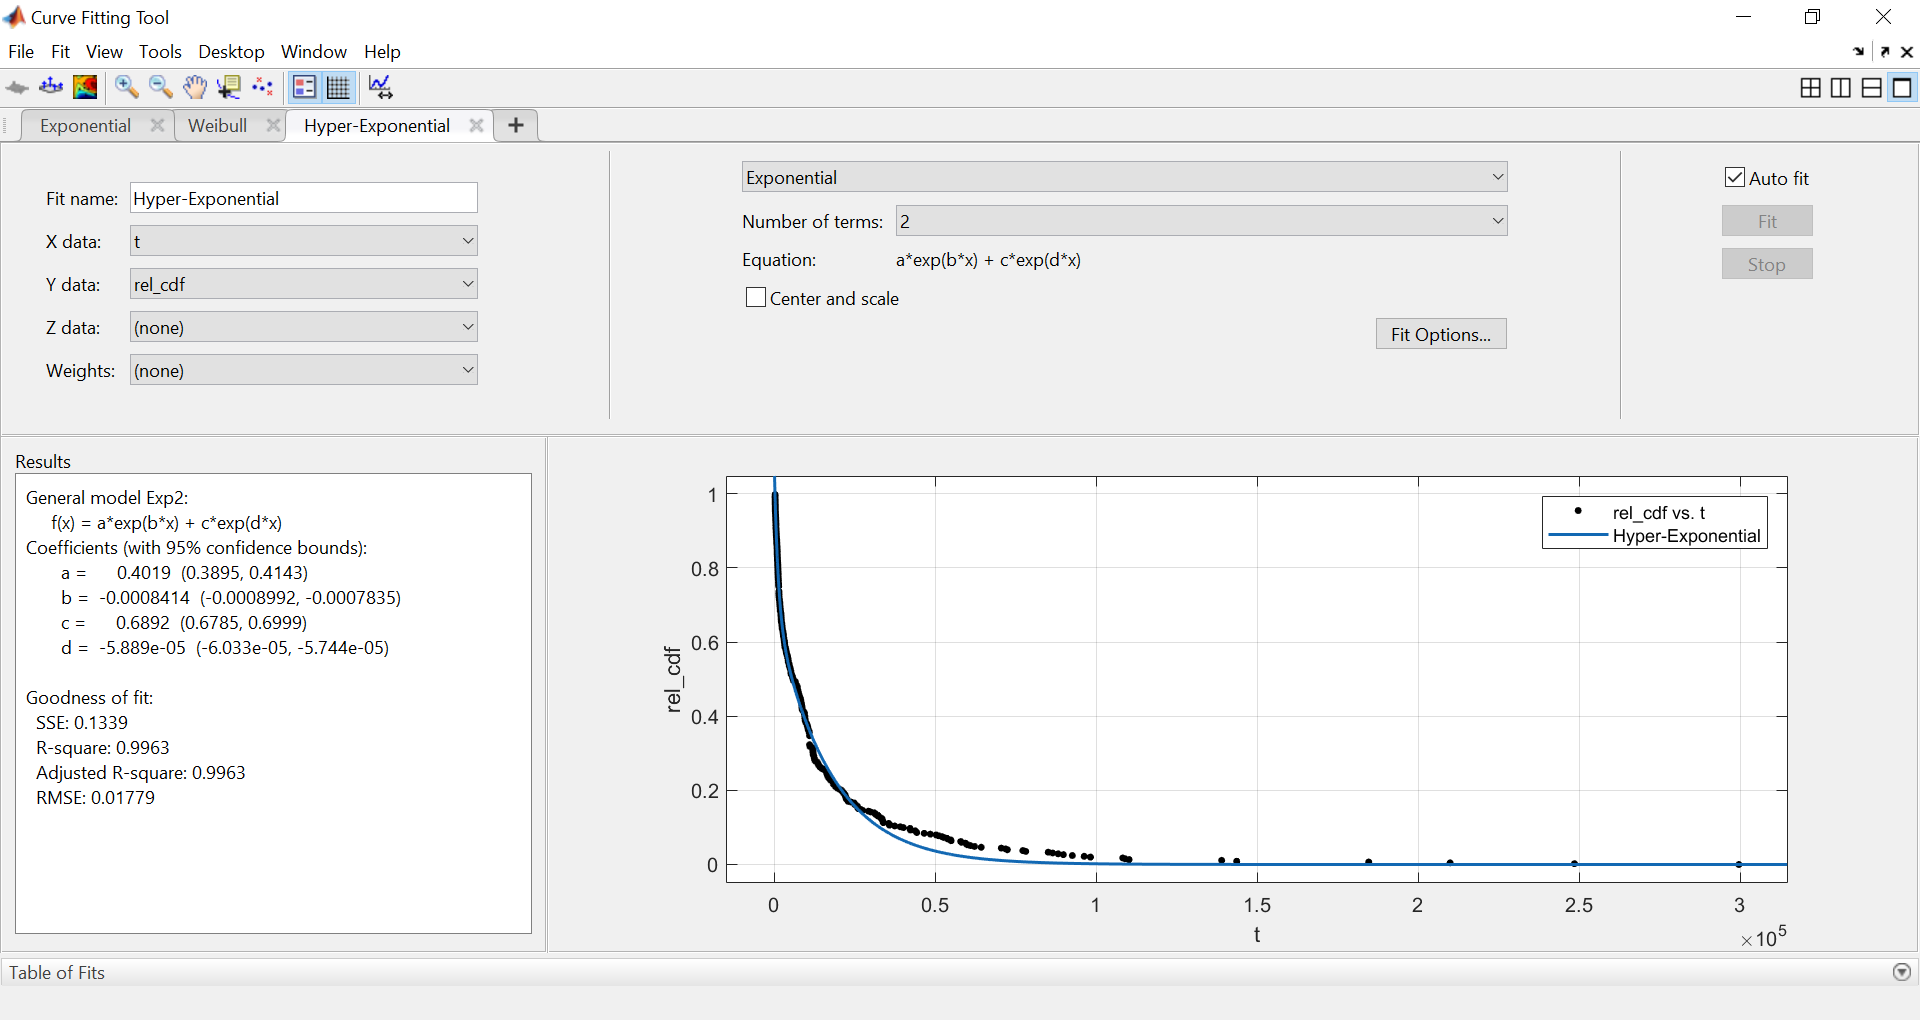
\includegraphics[width=0.9\linewidth,keepaspectratio]{HyperExponential_mercury}
    \caption{Curve Fitting modello esponenziale}
    \label{HyperExponential_mercury}
  \end{figure}

  Per valutare la bontà del fitting è stato utilizzato il \textbf{Kolmogorov-Smirnov Test}.\\

  \begin{figure}[!htbp]
    \centering
    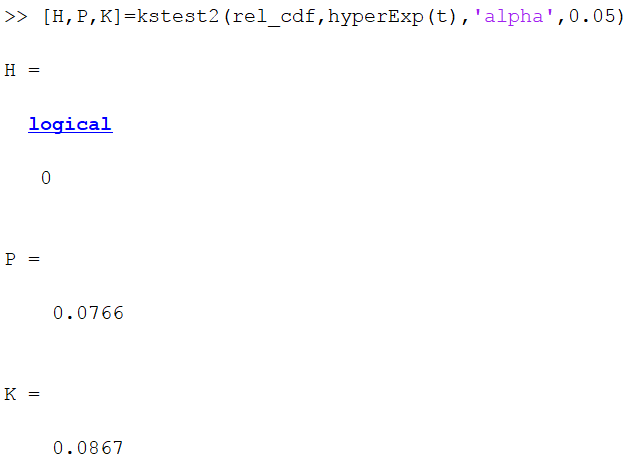
\includegraphics[width=0.5\linewidth,keepaspectratio]{ks_hyperexp_mercury}
    \caption{Kolmogorov-Smirnov Test Weibull}
    \label{ks_hyperexp_mercury}
  \end{figure}

  L'ipotesi non è rigettata al 7,66\% con un intervallo di confidenza al 95\%.\\

  \clearpage
\end{itemize}

Confrontando gli R-quadro di tutti i modelli utilizzati, il migliore risulta essere l'
\textbf{Iperesponenziale} anche se dal \textbf{Kolmogorov-Smirnov Test} l'unico
a non rigettare $H_0"$ il modello \textbf{Weibull}.\\

\clearpage

\section{Blue Gene L}
Blue Gene L è un super-calcolare IBM.\\
I nodi che compongono il sistema riportati nel log sono:
\begin{itemize}
  \item \textbf{Rack}: individuato nel log con la lettera R seguita da un numero,
  rappresenta la cabina contenente i nodi.\\
  \item \textbf{Nodo}: individuato nel log con la lettera N seguita da numero,
  reppresenta il blade del Rack contenente più Compute Card;
  \item \textbf{Compute Card}: individuata nel log con la lettera J seguita da un
  numero compreso tra 1 e 16;
  \item \textbf{Compute Chip}: individuati nel log come U01 e U11, ne sono presenti
  due per ogni Compute Card;
  \item \textbf{I-O Card}: individuata nel log come J18 ed è presente solo in alcuni
  nodi(N0,N4,N8,NC).
\end{itemize}

Il log è formato dai seguenti campi:
\begin{itemize}
  \item \textbf{Timestamp};
  \item \textbf{Nodo Origine};
  \item \textbf{Card Origine};
  \item \textbf{Messaggio}.
\end{itemize}

\subsection{Finestra di Coalescenza - CWIN}
La finestra di coalescence, definita in secondi, definisce un intervallo temporale
in cui cadono tutti gli eventi che vi appartengono.\\
Lo script \textbf{tupleCount\_func\_CWINpy.sh}(riportato in figura \ref{coalescence_window_mercury}), con input i file \textit{MercuryErrorLog.txt}
e \textit{tentative-CWIN.txt}, è stato utilizzato per calcolare il numero di tuple al
variare della dimensione della finestra di coalescenza.\\

\begin{figure}[!htbp]
  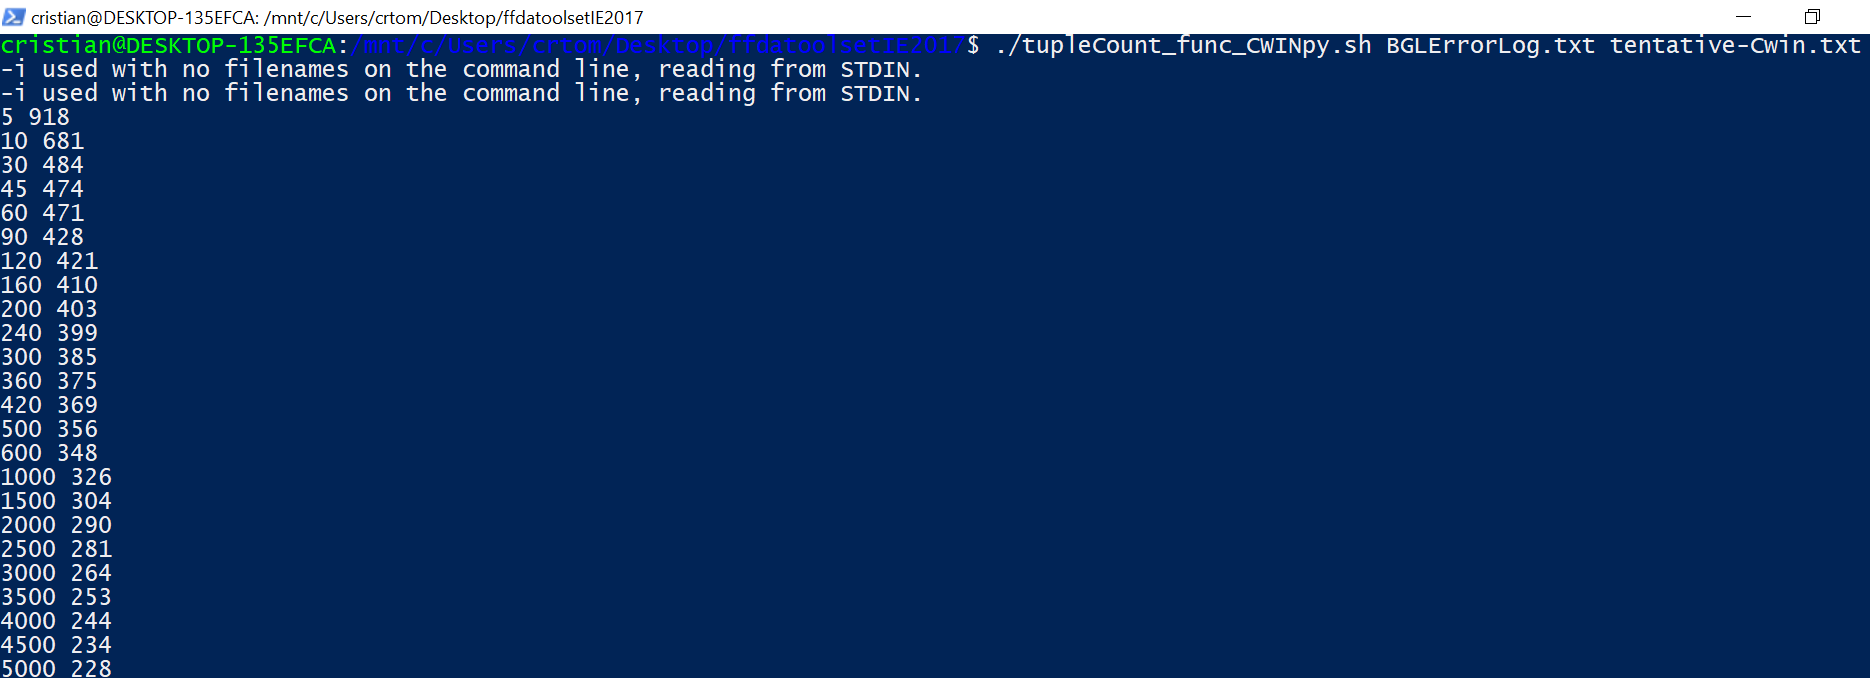
\includegraphics[width=1\linewidth,keepaspectratio]{coalescence_window_bgl}
  \caption{Script conteggio tuple al variare della finestra di coalescenza}
  \label{coalescence_window_bgl}
\end{figure}

\clearpage

L'output di tale script, plottato in matlab e presente in figura \ref{plot_coalescence_window_mercury},
è infine utilizzato per determinare un singolo valore di CWIN, ottenuto
considerando il punto successivo al ginocchio(knee) della curva.\\
Il valore di CWIN scelto è 300.\\
\begin{figure}[!htbp]
  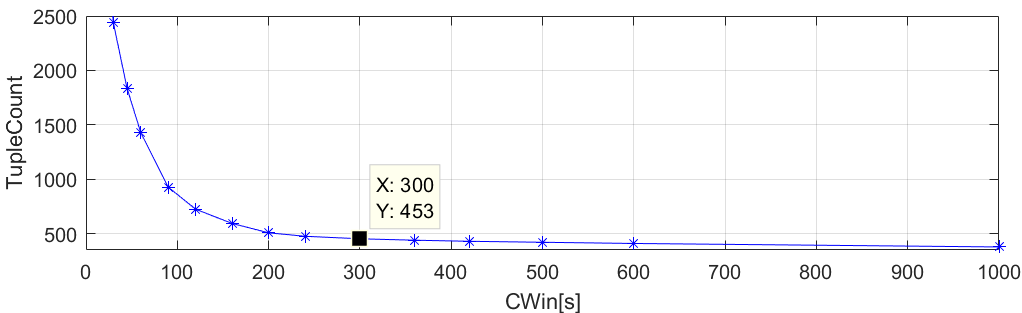
\includegraphics[width=1\linewidth,keepaspectratio]{plot_coalescence_window_mercury}
  \caption{Plot finestre di coalescenza}
  \label{plot_coalescence_window_mercury}
\end{figure}

Lo script bash \textbf{tupling\_with\_CWIN.sh} suddivide le righe del file di log
secondo la finestra di coalescenza calcolando infine per ogni tupla si seguenti parametri:

\begin{itemize}
  \item \textbf{Starting Points}: il timestamp della prima riga di ogni tupla generata;
  \item \textbf{Interarrivals}: il tempo che intercorre, tra due tuple consecutive, tra l'ultimo
  della prima tupla e il primo della seconda;
  \item \textbf{Lenghts}: il numero di righe di ogni tupla.
\end{itemize}

Analizzando il file \textbf{interarrivals.txt} in matlab tramite lo script \textbf{ttf\_ref}
si ottiene la CDF empirica della TTF(Time To Failure) e dualmente la Reliability (1-TTF).\\
In figura è riportato il grafico delle due CDF.

\begin{figure}[!htbp]
  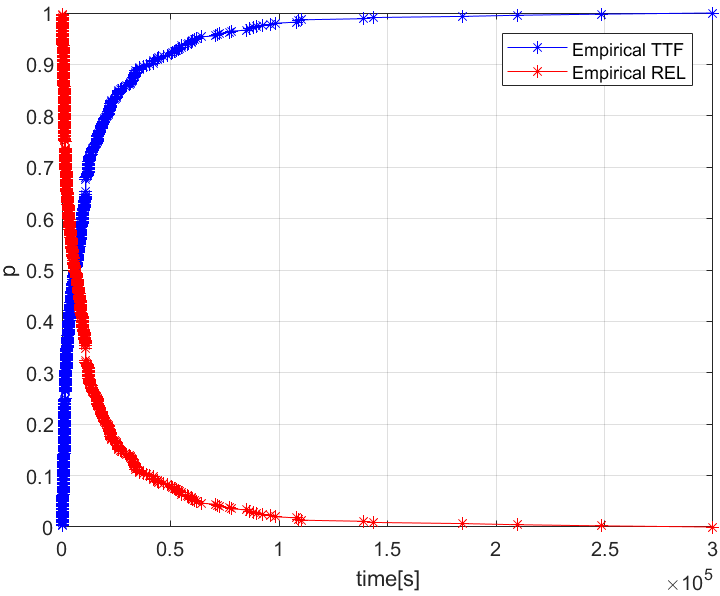
\includegraphics[width=1\linewidth,keepaspectratio]{ttf_rel_mercury}
  \caption{Plot TTF e Reliability}
  \label{ttf_rel_mercury}
\end{figure}

\section{Curve Fitting}

Dopo aver ottenuto la CDF della reliability è possibile procedere con fitting.\\
Utilizzando il tool di matlab \textbf{Curve Fitting} è stato possibile
analizzare i seguenti modelli:

\clearpage

\begin{itemize}
  \item \textbf{Esponenziale}:
  $$ y = e^{- \lambda  x} $$
  Il valore $\lambda$ è stato inizializzato a $1/MTTF$.\\
  Il modello risultante in matlab è riportato nella figura \ref{Exponential_mercury}.\\

  \begin{figure}[!htbp]
    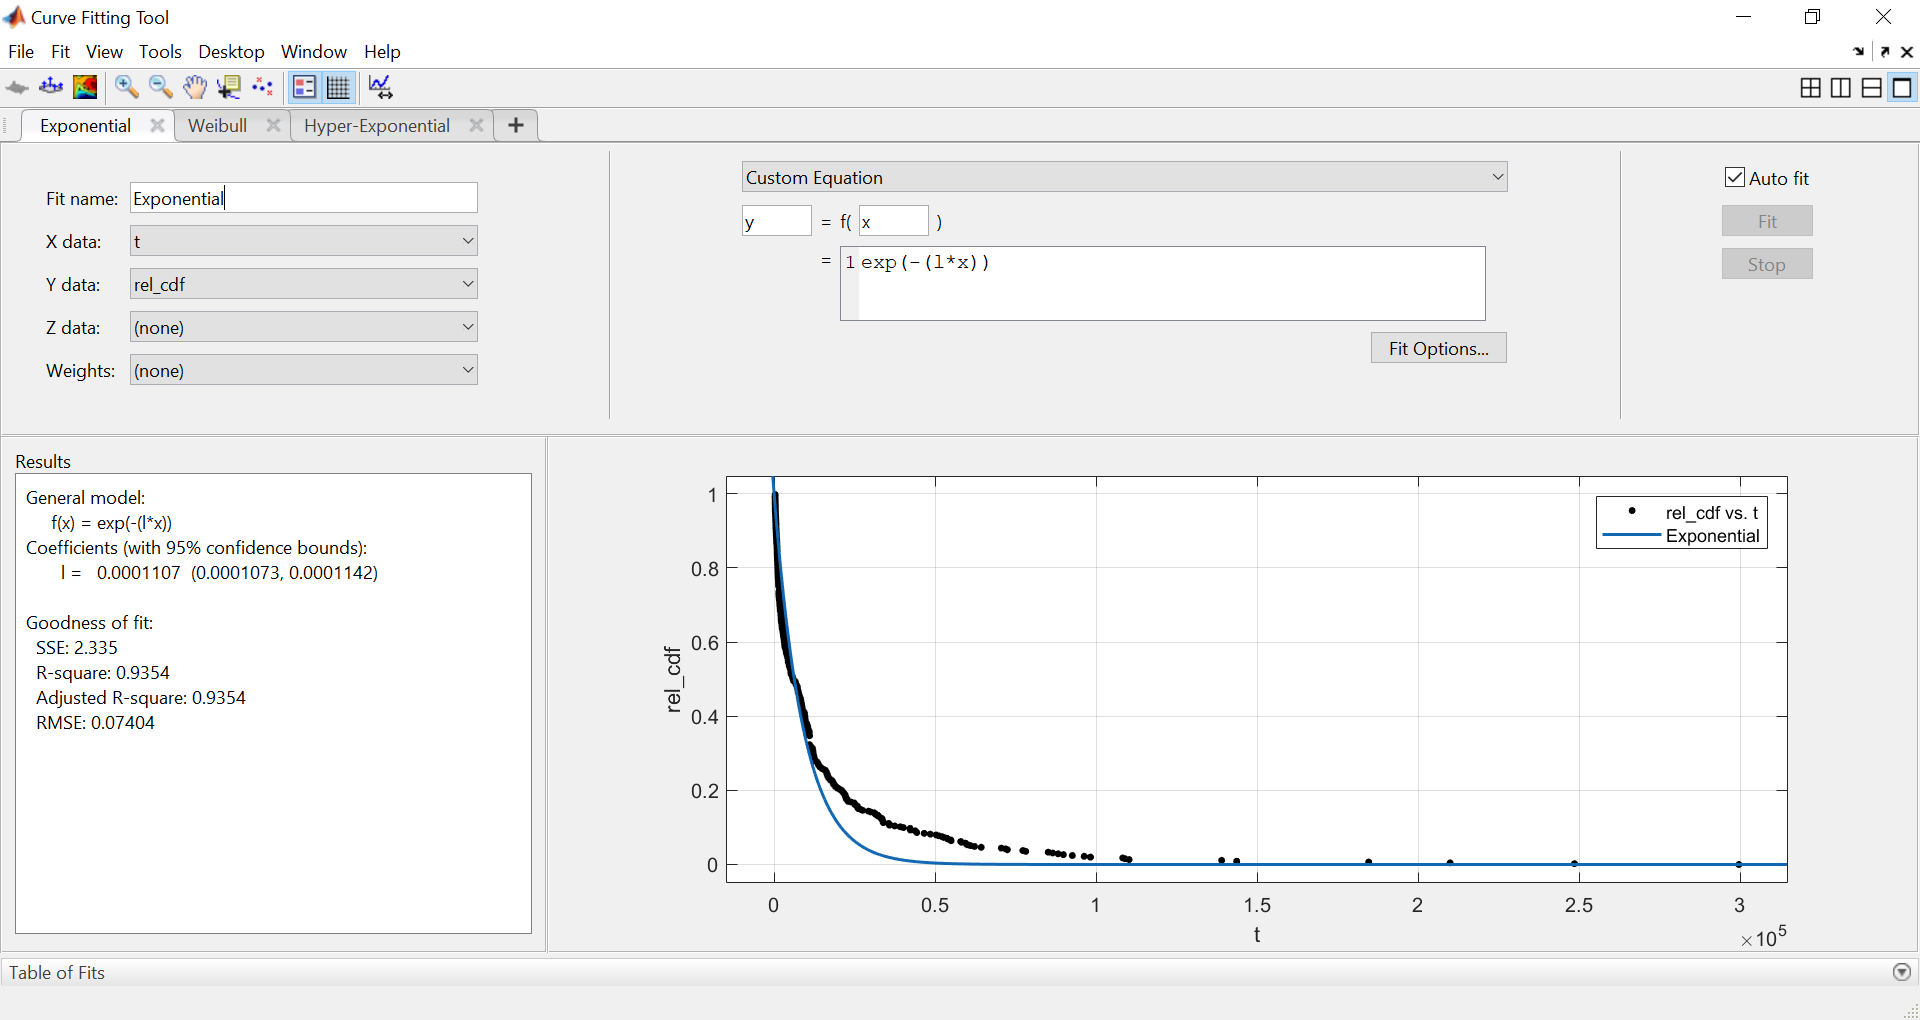
\includegraphics[width=.9\linewidth,keepaspectratio]{Exponential_mercury}
    \caption{Curve Fitting modello esponenziale}
    \label{Exponential_mercury}
  \end{figure}

  Per valutare la bontà del fitting è stato utilizzato il \textbf{Kolmogorov-Smirnov Test}.\\

  \begin{figure}[!htbp]
    \centering
    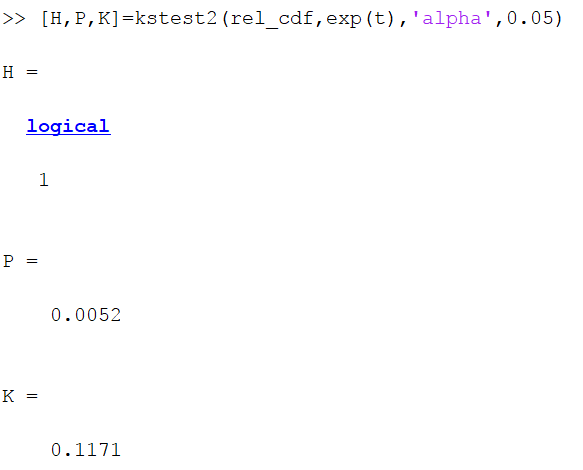
\includegraphics[width=0.5\linewidth,keepaspectratio]{ks_exp_mercury}
    \caption{Kolmogorov-Smirnov Test esponenziale}
    \label{ks_exp_mercury}
  \end{figure}

  L'ipotesi nulla è rigettata al 99,48\% con un intervallo di confidenza al 95\%.

  \clearpage

  \item \textbf{Weibull}:
  $$ y = e^{- (\lambda x)^\alpha} $$
  Il modello risultante in matlab è riportato nella figura \ref{Weibull_mercury}.\\
  \begin{figure}[!htbp]
    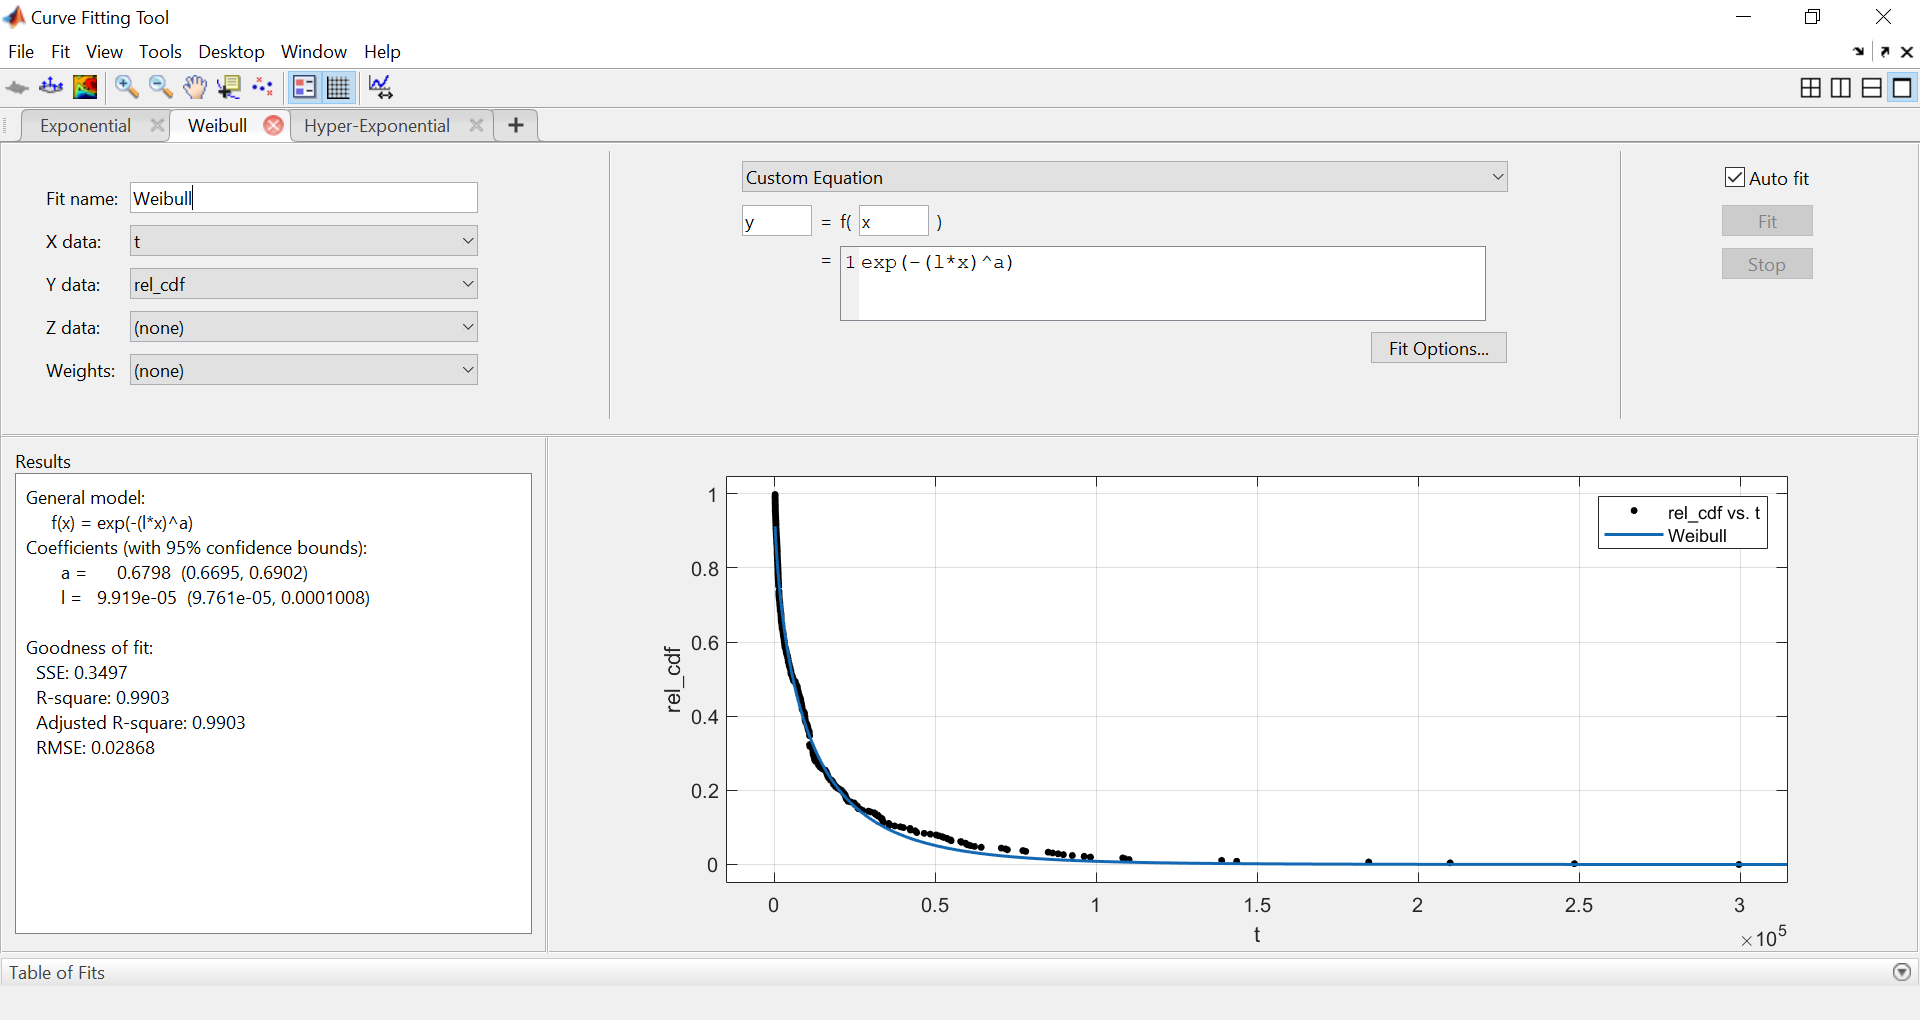
\includegraphics[width=0.9\linewidth,keepaspectratio]{Weibull_mercury}
    \caption{Curve Fitting modello esponenziale}
    \label{Weibull_mercury}
  \end{figure}

  Per valutare la bontà del fitting è stato utilizzato il \textbf{Kolmogorov-Smirnov Test}.\\

  \begin{figure}[!htbp]
    \centering
    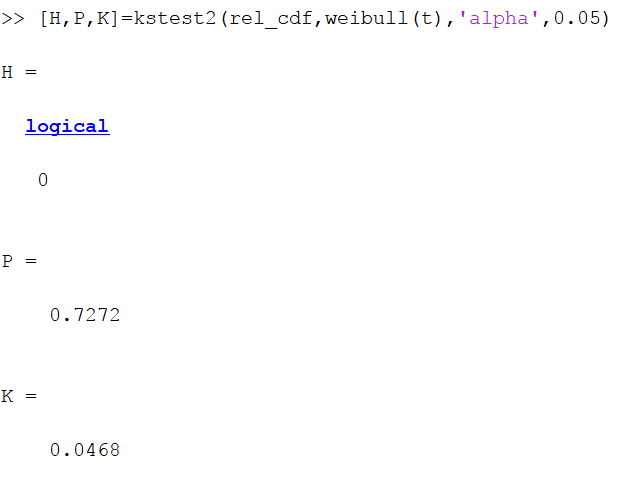
\includegraphics[width=0.5\linewidth,keepaspectratio]{ks_weibull_mercury}
    \caption{Kolmogorov-Smirnov Test Weibull}
    \label{ks_weibull_mercury}
  \end{figure}

  L'ipotesi nulla non è rigettata al 72,72\% con un intervallo di confidenza al
  95\% quindi osservando il anche il valore di R-quadro si può concludere che il
  modello ipotizzato fitta bene la CDF empirica.\\

  \clearpage

  \item \textbf{Iperesponenziale}:
  $$ y = a e^{- \lambda_1  x} +  b  e^{- \lambda_2  x} $$
  Il modello risultante in matlab è riportato nella figura \ref{HyperExponential_mercury}.\\

  \begin{figure}[!htbp]
    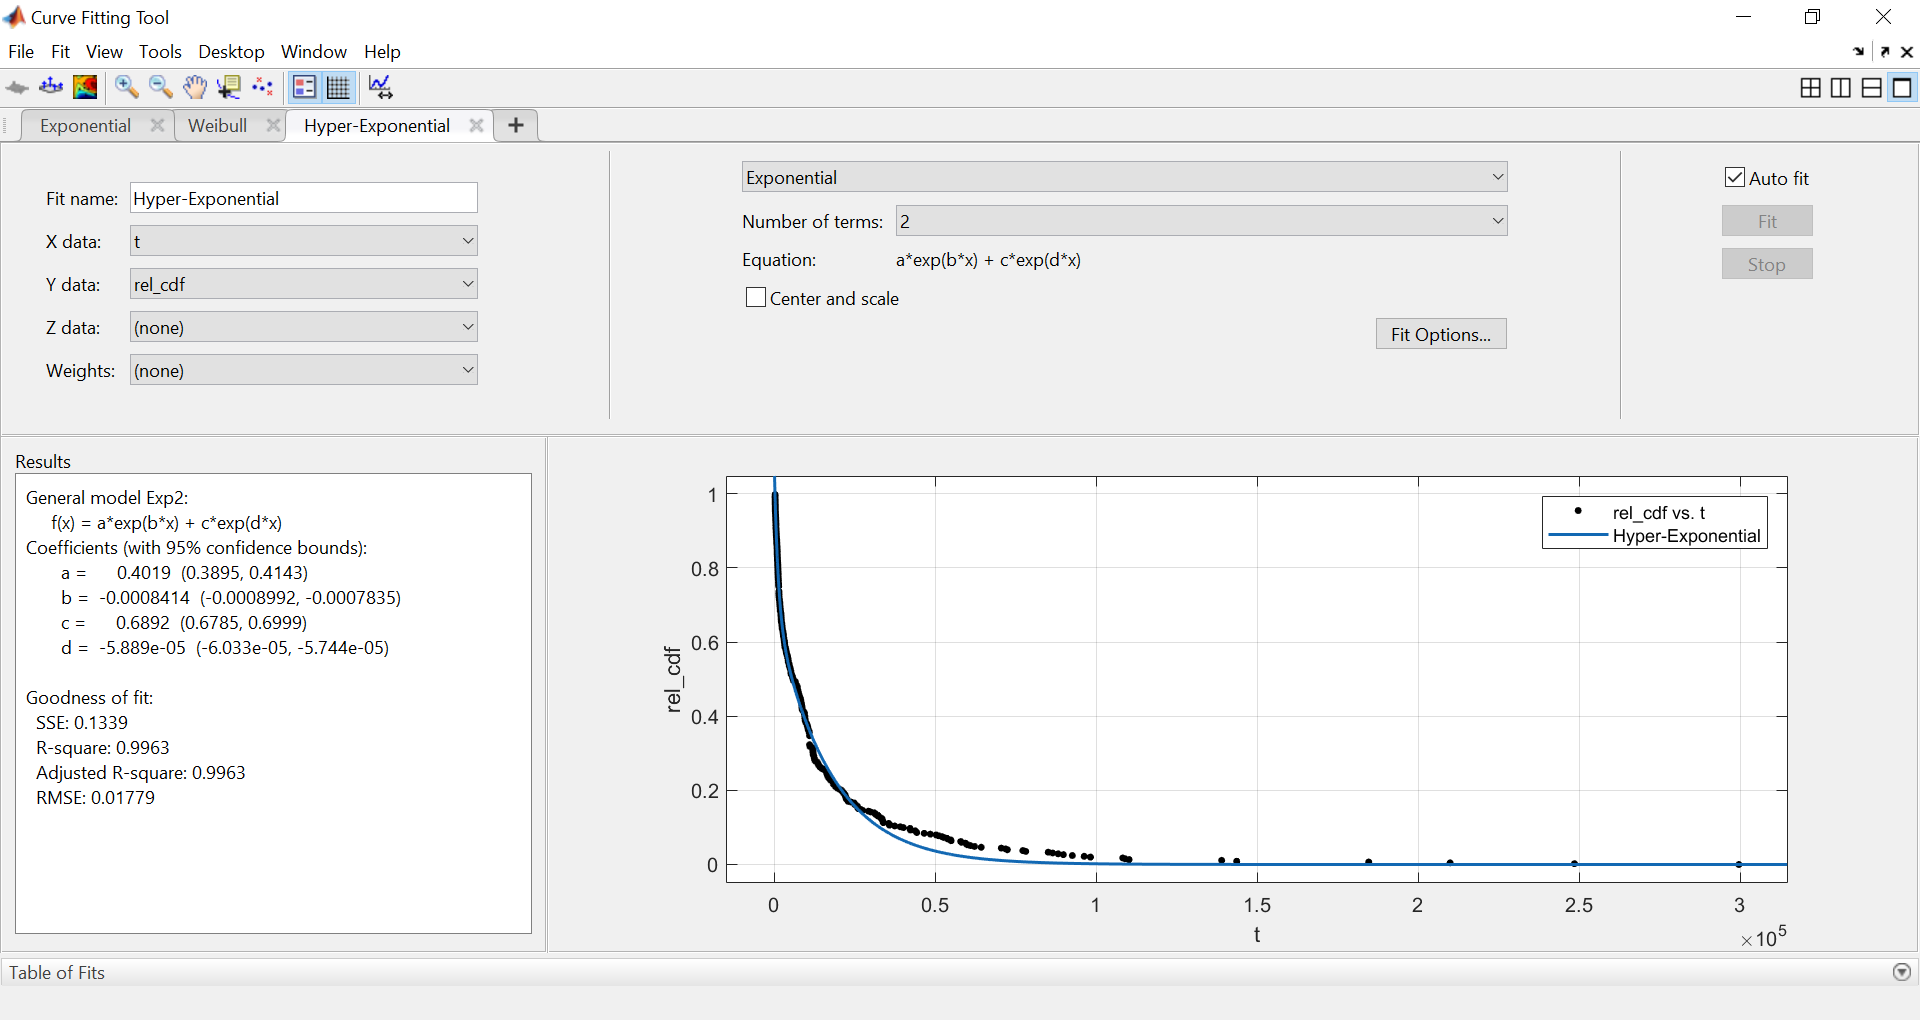
\includegraphics[width=0.9\linewidth,keepaspectratio]{HyperExponential_mercury}
    \caption{Curve Fitting modello esponenziale}
    \label{HyperExponential_mercury}
  \end{figure}

  Per valutare la bontà del fitting è stato utilizzato il \textbf{Kolmogorov-Smirnov Test}.\\

  \begin{figure}[!htbp]
    \centering
    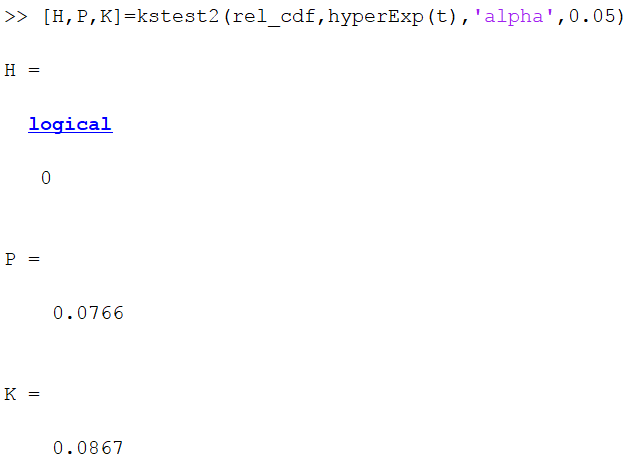
\includegraphics[width=0.5\linewidth,keepaspectratio]{ks_hyperexp_mercury}
    \caption{Kolmogorov-Smirnov Test Weibull}
    \label{ks_hyperexp_mercury}
  \end{figure}

  L'ipotesi non è rigettata al 7,66\% con un intervallo di confidenza al 95\%.\\

  \clearpage
\end{itemize}

Confrontando gli R-quadro di tutti i modelli utilizzati, il migliore risulta essere l'
\textbf{Iperesponenziale} anche se dal \textbf{Kolmogorov-Smirnov Test} l'unico
a non rigettare $H_0"$ il modello \textbf{Weibull}.\\
